% debut d'un fichier latex standard
\documentclass[a4paper,12pt,twoside]{article}
% Tout ce qui suit le symbole "%" est un commentaire
% Le symbole "\" désigne une commande LaTeX

% pour l'inclusion de figures en eps,pdf,jpg, png
\usepackage{graphicx}

% quelques symboles mathematiques en plus
\usepackage{amsmath}

% le tout en langue francaise
\usepackage[french]{babel}

% on peut ecrire directement les caracteres avec l'accent
%    a utiliser sur Linux/Windows (! dépend de votre éditeur !)
%\usepackage[utf8]{inputenc} % 
%\usepackage[latin1]{inputenc} % Pour Kile
\usepackage[T1]{fontenc}

%    a utiliser sur le Mac ???
%\usepackage[applemac]{inputenc}

% pour l'inclusion de liens dans le document 
\usepackage[colorlinks,bookmarks=false,linkcolor=blue,urlcolor=blue]{hyperref}
\usepackage{wrapfig}
\usepackage{subcaption}
\usepackage{caption}
\usepackage{float}

\paperheight=297mm
\paperwidth=210mm

\setlength{\textheight}{235mm}
\setlength{\topmargin}{-1.2cm} % pour centrer la page verticalement
%\setlength{\footskip}{5mm}
\setlength{\textwidth}{16.5cm}
\setlength{\oddsidemargin}{0.0cm}
\setlength{\evensidemargin}{-0.3cm}

\pagestyle{plain}

% nouvelles commandes LaTeX, utilis\'ees comme abreviations utiles
\def \be {\begin{equation}}
\def \ee {\end{equation}}
\def \dd  {{\rm d}}

\newcommand{\mail}[1]{{\href{mailto:#1}{#1}}}
\newcommand{\ftplink}[1]{{\href{ftp://#1}{#1}}}
%
% latex SqueletteRapport.tex      % compile la source LaTeX
% xdvi SqueletteRapport.dvi &     % visualise le resultat
% dvips -t a4 -o SqueletteRapport.ps SqueletteRapport % produit un PostScript
% ps2pdf SqueletteRapport.ps      % convertit en pdf

% pdflatex SqueletteRapport.pdf    % compile et produit un pdf

% ======= Le document commence ici ================================

\begin{document}

% Le titre, l'auteur et la date
\title{Physique numérique Exercice 1}
\author{Armand Le Douarec, Maxime Chatelin\\  % \\ pour fin de ligne
{\small \mail{armand.ledouarec@epfl.ch}, \mail{maxime.chatelin@epfl.ch}}}
\date{\today}\maketitle
\tableofcontents % Table des matieres

% Quelques options pour les espacements entre lignes, l'indentation 
% des nouveaux paragraphes, et l'espacement entre paragraphes
\baselineskip=16pt
\parindent=0pt
\parskip=12pt

\section{Introduction}

Dans cette étude, nous analysons numériquement le comportement d'un satellite soumis aux forces gravitationnelles de la Terre et de la Lune, ainsi qu'aux effets inertiels, notamment la force de Coriolis. En considérant un modèle simplifié à trois corps avec une masse négligeable du satellite, nous implémentons et comparons trois méthodes numériques de résolution des équations du mouvement : les schémas d'Euler explicite, implicite et semi-implicite. L'objectif est d'évaluer la stabilité et la précision de ces méthodes, notamment en ce qui concerne la conservation de l'énergie mécanique et la fidélité des trajectoires simulées.

\section{Calculs analytiques}

\subsection{Positions de la Terre et de la Lune dans le référentiel $R'$ et position d'équigravité}
Soient $m_T$ et $m_L$ les masses de la Terre et de la Lune. Soient $x'_T$ et $x'_L$ les positions de la Terre et de la Lune dans le référentiel $R'$ avec pour système de coordonnées $Gx'y'$ cartésien. Le centre de masse $G$ est défini par:\\

\begin{equation}
G = \displaystyle \frac{m_Tx'_T+m_Lx'_L}{m_T+m_L}
\end{equation}

D'après la définition du référentiel $R'$, on a $G = 0$. De plus, on définit la distance Terre-Lune par $d_{TL}=x'_L-x'_T$. On obtient le système suivant:\\

\begin{equation}
\left\{
\begin{tabular}{l}
    $\displaystyle \frac{m_Tx'_T+m_Lx'_L}{m_T+m_L} = 0$ \\[8pt]
    $x'_L - x'_T = d_{TL}$
\end{tabular}
\right.
\Rightarrow
\left\{
\begin{tabular}{l}
    $x'_T = -\displaystyle \frac{m_L}{m_T} x'_L$ \\[8pt]
    $x'_L - x'_T = d_{TL}$
\end{tabular}
\right.
\Rightarrow
\left\{
\begin{tabular}{l}
    $x_T = -\displaystyle \frac{m_Ld_{TL}}{m_T+m_L}$ \\[8pt]
    $x_L = \displaystyle \frac{m_Td_{TL}}{m_T+m_L}$
\end{tabular}
\right.
\end{equation}

Soit $G_{grav}$ la constante de gravitation. La position du point d'équigravité $x'_0$ est donnée par la solution de l'équation suivante (somme des forces gravitationnelles nulles):
\begin{equation}
-G_{grav}\displaystyle \frac{m_L}{(x'_L-x'_0)^2} + G_{grav}\displaystyle \frac{m_T}{(x'_T-x'_0)^2} = 0
\end{equation}
\begin{equation}
\Rightarrow
m_L(x'_T-x'_0)^2-m_T(x'_L-x'_0)^2=0
\end{equation}
\begin{equation}
\Rightarrow
(x'_T\sqrt{m_L}-x'_L\sqrt{m_T}+x'_0(\sqrt{m_T}-\sqrt{m_L}))(-x'_0(\sqrt{m_L}+\sqrt{m_T})+x'_T\sqrt{m_L}+x'_L\sqrt{m_T})=0
\end{equation}
\begin{equation}
\Rightarrow
x'_0 = \displaystyle\frac{x'_T\sqrt{m_L}-x'_L\sqrt{m_T}}{\sqrt{m_L}-\sqrt{m_T}} \quad \text{ou} \quad x'_0 =\displaystyle\frac{x'_T\sqrt{m_L}+x'_L\sqrt{m_T}}{\sqrt{m_L}+\sqrt{m_T}}
\end{equation}
La solution physique, celle qui nous intéresse, est la suivante :
\begin{equation}
x'_0 =\displaystyle\frac{x'_T\sqrt{m_L}+x'_L\sqrt{m_T}}{\sqrt{m_L}+\sqrt{m_T}}
\end{equation}
En effet, l'autre solution ne se situe pas entre la Terre et la Lune, due au changement de l'orientation de la force gravitationnelle.

\subsection{Vitesse angulaire du référentiel $R'$}

Soit $\Omega$ la vitesse angulaire du référentiel $R'$. En effectuant le bilan des forces dans $R'$ et en tenant compte de l'inertie de la Lune et de la Terre dans ce référentiel. On obtient l'équation suivante:
\begin{equation}
0 = -\displaystyle\frac{G_{grav}m_Tm_L}{{d_{TL}}^2} + m_L\Omega^2x_L
\quad\Rightarrow\quad
\Omega = \sqrt{\displaystyle\frac{G_{grav}m_T}{{d_{TL}}^2x_L}}
\end{equation}

\subsection{Système d’équations différentielles du mouvement du satellite dans le référentiel $R'$}

Soit $\vec{y}$ le vecteur défini par $\vec{y} = (v'_x,v'_y,x',y')$. Il représente les vecteurs vitesse et position du satellite. Soit $m_S$ la masse du satellite. Soit $\vec{F_{R'}} \equiv (F_{x,R'},F_{y,R'})$. On a:
\begin{equation}
\vec{F_{R'}} = \vec{F}_{grav}+\vec{F}_{Coriolis}+\vec{F}_{centrifuge}
\end{equation}
avec l'expression de ces forces:
\begin{equation}
\vec{F}_{grav} = -\displaystyle\frac{G_{grav}m_Tm_S}{(x'-x'_T)^2+{y'}^2}\vec{e}_{TS} -\displaystyle\frac{G_{grav}m_Lm_S}{(x'-x'_L)^2+{y'}^2}\vec{e}_{LS} 
\end{equation}
\begin{equation}
\vec{F}_{Coriolis} = -2m_S\vec{\Omega}\times\vec{v} \quad \vec{F}_{centrifuge}=m_S\vec{\Omega}\times(\vec{\Omega}\times\vec{GS})
\end{equation}
avec $\vec{e}_{TS}$ le vecteur unitaire orienté de la Terre vers le satellite, $\vec{e}_{LS}$ le vecteur unitaire orienté de la Lune vers le satellite et $\vec{GS}$ le vecteur position du satellite dans le référentiel $R'$.
\begin{equation}
\displaystyle\frac{\text{d}\vec{y}}{\text{d}t} = \vec{f}(\vec{y}) = \left(
\begin{tabular}{c}
     $\frac{F_{x,R'}}{m_S}$ \\
     $\frac{F_{y,R'}}{m_S}$\\
     $v'_x$\\
     $v'_y$
\end{tabular}
\right)
\end{equation}

En projetant $\vec{F_{R'}}$ sur chaque axe du système de coordonnées, on obtient l'équation finale:

\begin{equation}
\displaystyle\frac{\text{d}\vec{y}}{\text{d}t}= \left(
\begin{tabular}{c}
     $-\left(\frac{G_{grav}m_T}{(x'-x'_T)^2+{y'}^2}+\frac{G_{grav}m_L}{(x'-x'_L)^2+{y'}^2}\right)\left(\frac{x'}{\sqrt{{x'}^2+{y'}^2}}\right)+ \Omega^2x' + 2\Omega v'_y$ \\
     $-\left(\frac{G_{grav}m_T}{(x'-x'_T)^2+{y'}^2}+\frac{G_{grav}m_L}{(x'-x'_L)^2+{y'}^2}\right)\left(\frac{y'}{\sqrt{{x'}^2+{y'}^2}}\right)+ \Omega^2y' - 2\Omega v'_x$\\
     $v'_x$\\
     $v'_y$
\end{tabular}
\right)
\end{equation}

\subsection{Énergie mécanique}

L'énergie mécanique $E_{mec}$ est la suivante:

\begin{equation}
E_{mec} = \displaystyle\frac{1}{2}m_S\left({v'_x}^2+{v'_y}^2\right)-\displaystyle\frac{G_{grav}m_Tm_S}{\sqrt{(x'-x'_T)^2+{y'}^2}}-\displaystyle\frac{G_{grav}m_Lm_S}{\sqrt{(x'-x'_L)^2+{y'}^2}}
 - \displaystyle\frac{1}{2}m_S\Omega^2{GS}^2
 \end{equation}

L'énergie mécanique est conservée car la puissance des forces non conservatives est nulle. En effet, en analysant chaque force, on a:
\begin{equation}
\vec{F'} = \vec{F}_{gravitationnel}+\vec{F}_{Coriolis}+\vec{F}_{centrifuge}
\end{equation}
avec $\vec{F}_{gravitationnel}$ conservative par propriété de la force gravitationnelle. Pour la puissance de la force de Coriolis, on a:
\begin{equation}
P_{Coriolis} = \vec{F}_{Coriolis}. \vec{v} = -2m_S(\vec{\Omega}\times\vec{v}).\vec{v} = 0
\end{equation}
Tandis que pour la force centrifuge, on a:
\begin{equation}
\vec{F}_{centrifuge} = -m_S\vec{\Omega}\times(\vec{\Omega}\times\vec{GS)}= m_S\Omega^2\vec{GS}
\end{equation}
or, d'après le théorème de Stokes, pour toute surface $A$:
\begin{equation}
\vec{F} \text{ conservative} \quad\Leftrightarrow\quad \oint_{\partial A}\vec{F}.\vec{\text{d}r} \quad\Leftrightarrow\quad \iint_{A}\left(\vec{\nabla}\times \vec{F}\right).\vec{\text{d}s}
\end{equation}

Or, ici $\vec{\nabla}\times \vec{F} = \vec{\nabla}\times (m_S\Omega^2\vec{GS}) = \vec{0}$\\

Donc la force centrifuge est conservative. On  en déduit ainsi que l'énergie mécanique est bien conservée.

\subsection{Analyse des forces exercées sur le satellite}

Au point d’équigravité, la somme des forces gravitationnelles exercées par la Terre et la Lune est nulle. Cependant, dans le référentiel tournant, le satellite subit une force d’inertie dirigée vers la Lune. Cette force est responsable de l’accélération initiale du satellite dans cette direction, ce qui le fait quitter son point d'équigravité, le rendant donc instable . Lorsque le satellite acquiert une vitesse non nulle, la force de Coriolis s'applique alors. Elle est perpendiculaire à la vitesse et tend à courber la trajectoire du satellite, et permet donc d'éviter au satellite d'entrer directement en collision avec la Lune.

\section{Implémentation en C++}

L'implémentation des schémas numériques est réalisée en C++. Nous définissons les équations différentielles du mouvement dans un référentiel tournant et utilisons une intégration discrète pour simuler la trajectoire du satellite.

\subsection{Définition des constantes et des structures de données}

Nous définissons d'abord les constantes physiques utilisées dans la première étape de la simulation, ainsi que les structures de données permettant de stocker les positions et vitesses du satellite.

\begin{verbatim}
// Constantes physiques
tfin   = 259200 
nsteps = 4000
G_grav = 6.6743e-11
mt     = 5.972e24
ml     = 7.348e22
rt     = 6378100 !metr
rl     = 1737100 ! metr
dist   = 385000000 ! metr 
tol    = 1e-3
alpha  = 0.5
maxit  = 100
vx0 = 0
vy0 = 0
x0 = 0
y0 = 0

\end{verbatim}

\subsection{Comparaison des 3 schémas pour un même nombre de pas de temps}
Nous implémentons trois variantes du schéma d'Euler pour un pas de temps $N_{steps}=4000$, le schéma implicite avec $\alpha=0$, le schéma semi-implicite avec $\alpha=0.5$ et le schéma explicite avec $\alpha=1$. Les résultats sont présentés dans la Fig.(\ref{fig1}). Les trois courbes commencent de façon similaire avant de se rapprocher de la Lune, puis on observe des différences majeures dans leur comportement:

\begin{figure}[H]
\begin{subfigure}{0.45\textwidth}  % Réduire la taille pour s'assurer qu'elles tiennent côte à côte
    \centering  % Centrer cette sous-figure
    \includegraphics[scale=0.45]{Figure_1.png}
\end{subfigure}
\hspace{0.05\textwidth}
\begin{subfigure}{0.45\textwidth}  % Réduire également ici
    \centering  % Centrer cette sous-figure
    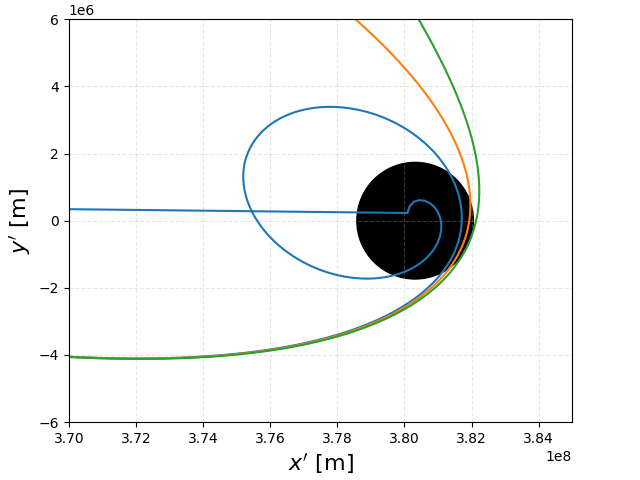
\includegraphics[scale=0.45]{Graphes/Trajectoire_zoom.png}
\end{subfigure}
\captionsetup{justification=centering}
\caption{Trajectoires du satellite pour $N_{steps} = 4000$, avec le schéma implicite en vert ($\alpha$ = 0), semi-implicite en orange ($\alpha$ = 0.5) et explicite en bleu ($\alpha$ = 1). On montre une image d'ensemble et une zoomée.}
\label{fig1}
\end{figure}

\vspace{-1cm}

Le schéma implicite fait tendre le satellite vers le centre de la Lune, ce qui l'accélère exponentiellement et puis d'un coup projette le satellite à l'horizon en ligne droite. Ce schéma est irréaliste car le satellite s'approche beaucoup trop de la Lune, jusqu'à clairement rentrer à l'intérieur de celle-ci, et l'utilise pour se projeter au loin.
Le schéma explicite s’éloigne plus de la lune, ce qui donne une courbe assez régulière au satellite, mais l'erreur est grande.
Le schéma semi-implicite offre un bon compromis en réduisant les erreurs sans sacrifier la stabilité. De plus, on trace l'énergie mécanique en fonction du temps et les résultats sont montrés dans la Fig.(\ref{fig2}).


\begin{figure}[H]
\centering
\begin{subfigure}{0.45\textwidth}  % Réduire la taille pour s'assurer qu'elles tiennent côte à côte
    \centering  % Centrer cette sous-figure
    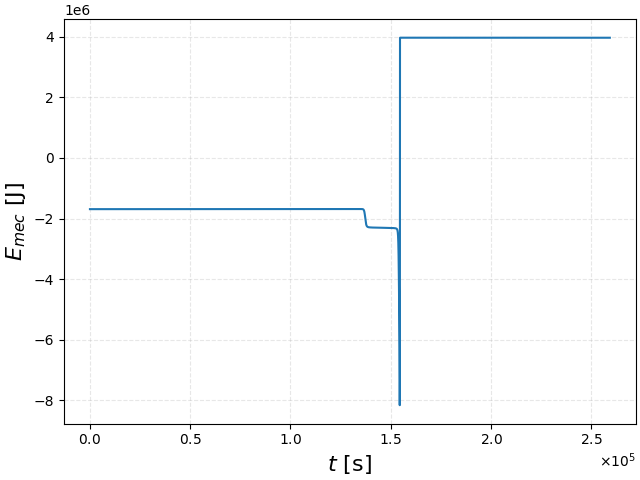
\includegraphics[scale=0.4]{Graphes/E_mec_alpha_0.png}
\end{subfigure}
\hspace{0.07\textwidth}
\begin{subfigure}{0.45\textwidth}  % Réduire également ici
    \centering  % Centrer cette sous-figure
    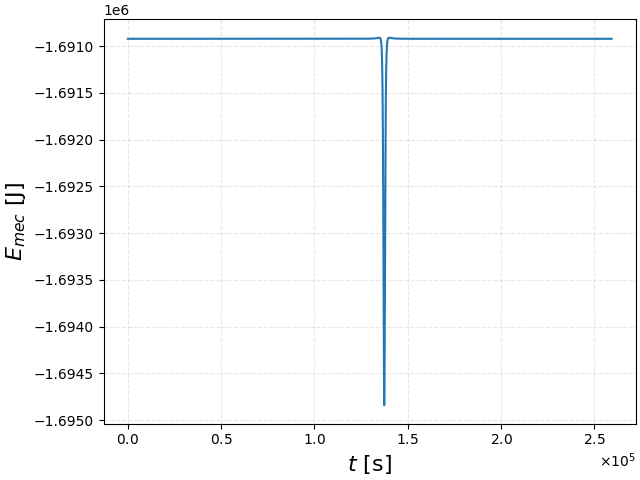
\includegraphics[scale=0.4]{Graphes/E_mec_alpha05.png}
\end{subfigure}
\begin{subfigure}{0.45\textwidth}  % Réduire la taille pour s'assurer qu'elles tiennent côte à côte
    \centering  % Centrer cette sous-figure
    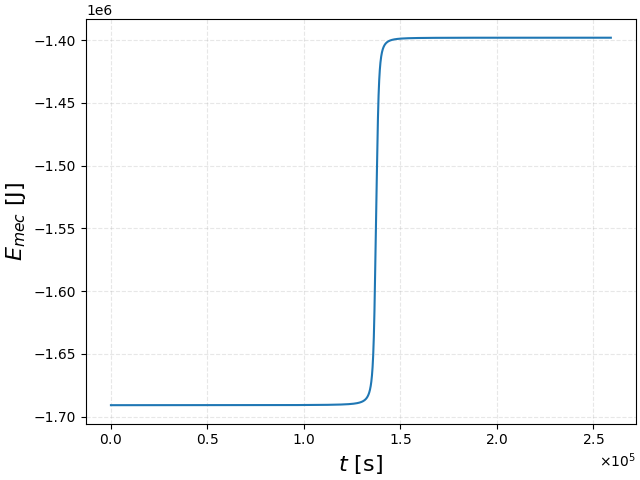
\includegraphics[scale=0.4]{Graphes/E_mec_alpha_1.png}
\end{subfigure}
\captionsetup{justification=centering}
\caption{Energie mécanique du satellite pour $N_{steps} = 4000$, avec le graphe du schéma implicite à gauche ($\alpha$ = 0), semi-implicite à droite ($\alpha$ = 0.5) et explicite en bas ($\alpha$ = 1).}
\label{fig2}
\end{figure}

\vspace{-1cm}

Pour le schéma implicite, l'énergie mécanique diminue légèrement jusqu'à augmenter subitement lorsqu'elle atteint le point critique expulsant le satellite vers l'infini. Le schéma explicite créé une erreur incongrue qui fait augmenter l'énergie mécanique alors qu'elle devrait rester constante. Enfin, le schéma semi-implicite a une erreur mécanique qui ne varie que très peu, surtout par rapport  aux deux autres schémas, ce qui montre une erreur marginalement faible.

On effectue ici les mêmes opérations pour $N_{steps}=40000$. Ce qui change ici, c'est que puisque l'écart entre deux pas de temps est divisé par dix, les écarts entre les trois schémas sont aussi diminués. En effet, la Fig.(\ref{fig3}) montre que le satellite évolue  similairement dans les trois schémas. Le schéma implicite n'expulse plus le satellite à l'infini à cause d'une trajectoire passant trop proche du centre de la Lune. Cependant, on voit toujours que le schéma implicite rapproche le satellite de la Lune, et c'est l'inverse pour le schéma explicite.

\vspace{-0.1cm}

\begin{figure}[H]
\begin{subfigure}{0.45\textwidth}  % Réduire la taille pour s'assurer qu'elles tiennent côte à côte
    \centering  % Centrer cette sous-figure
    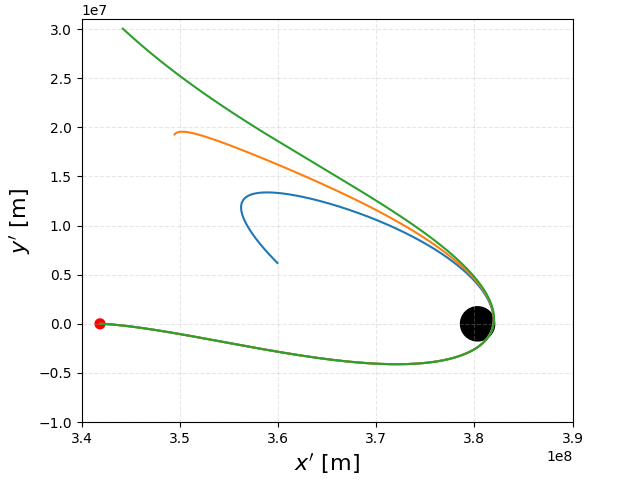
\includegraphics[scale=0.4]{Graphes/Trajectoire_2.png}
\end{subfigure}
\hspace{0.05\textwidth}
\begin{subfigure}{0.45\textwidth}  % Réduire également ici
    \centering  % Centrer cette sous-figure
    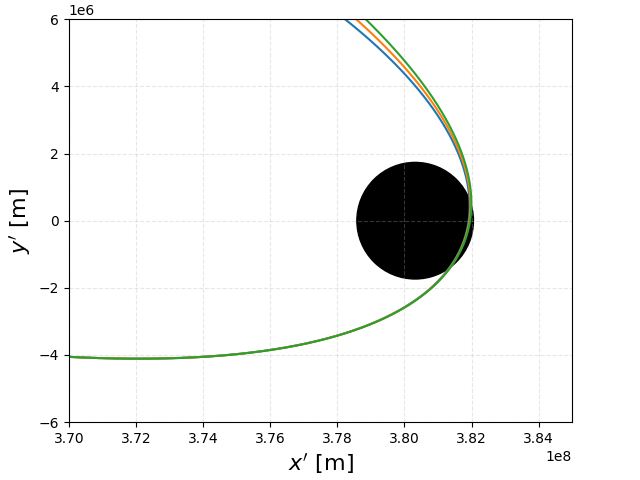
\includegraphics[scale=0.4]{Graphes/Trajectoire_zoom_2.png}
\end{subfigure}
\captionsetup{justification=centering}
\caption{Trajectoires du satellite pour $N_{steps} = 40000$, avec le schéma implicite en vert ($\alpha$ = 0), semi-implicite en orange ($\alpha$ = 0.5) et explicite en bleu ($\alpha$ = 1). On montre une image d'ensemble et une zoomée.}
\label{fig3}
\end{figure}
\vspace{-1cm}

Si on observe maintenant les traces temporelles de l'énergie mécanique présentées Fig.(\ref{fig4}), on voit que le schéma semi-implicite est meilleur en terme de conservation car l'énergie mécanique est mieux conservée que le schémas implicite (resp. explicite), qui la diminue (resp. l'augmente).




\begin{figure}[H]
    \centering
    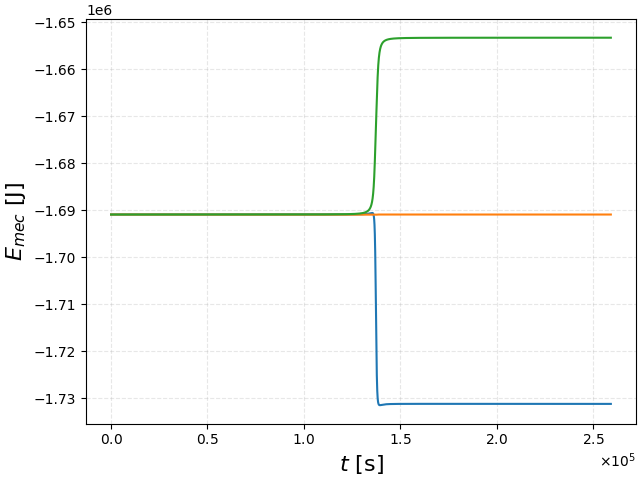
\includegraphics[width=0.48\textwidth]{Graphes/E_mec_2.png}
    \captionsetup{justification=centering}
    \caption{Énergie mécanique du satellite pour $N_{steps} = 40000$, avec le graphe du schéma implicite en bleu ($\alpha$ = 0), semi-implicite en orange ($\alpha$ = 0.5) et explicite en vert  ($\alpha$ = 1)}
    \label{fig4}
\end{figure}

\clearpage

\subsection{Etude de convergence des 3 schémas numériques}

Maintenant, on effectue des séries de simulations à différents $N_{steps}$ pour chaque schéma afin d'étudier la convergence. On prend $N_{steps}=[4, 6, 10, 14, 20, 50, 100] \times 10^3$, et on dresse les Fig.(\ref{fig5}) et Fig.(\ref{fig6}), qui représentent les positions finales de $x$ et de $y$ en fonction de $\Delta t$ élevé à une certaine puissance.

\begin{figure}[H]
\begin{subfigure}{0.45\textwidth}  % Réduire la taille pour s'assurer qu'elles tiennent côte à côte
    \centering  % Centrer cette sous-figure
    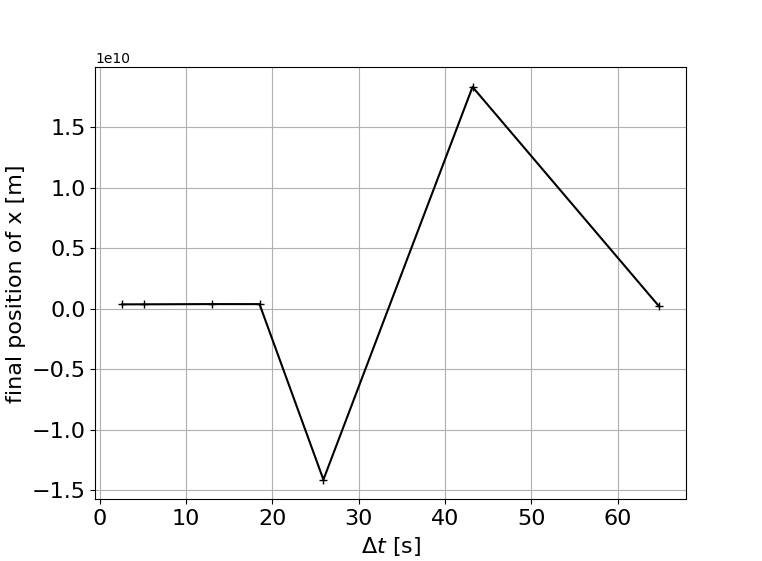
\includegraphics[scale=0.4]{Graphes/convergence_x_alpha_0.png}
    \captionsetup{justification = centering, font=large}
    \caption{}
\end{subfigure}
\hspace{0.05\textwidth}
\begin{subfigure}{0.45\textwidth}  % Réduire également ici
    \centering  % Centrer cette sous-figure
    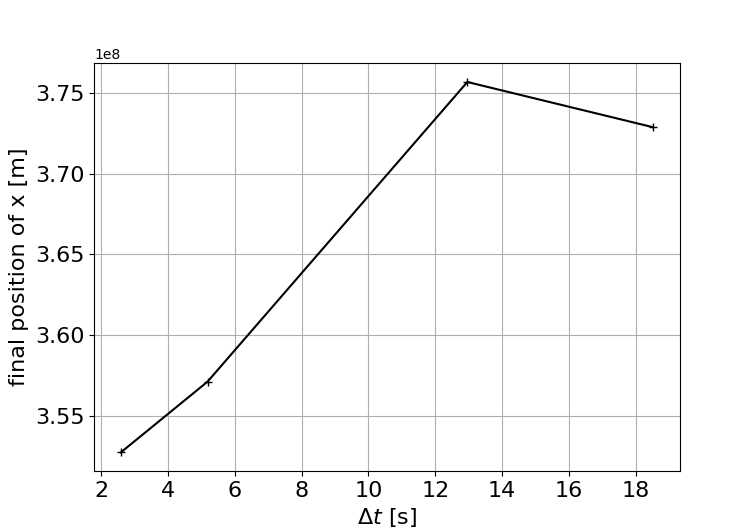
\includegraphics[scale=0.42]{Graphes/convergence_x_alpha_0_zoom.png}
    \captionsetup{justification = centering, font=large}
    \caption{}
\end{subfigure}
\begin{subfigure}{0.45\textwidth}  % Réduire la taille pour s'assurer qu'elles tiennent côte à côte
    \centering  % Centrer cette sous-figure
    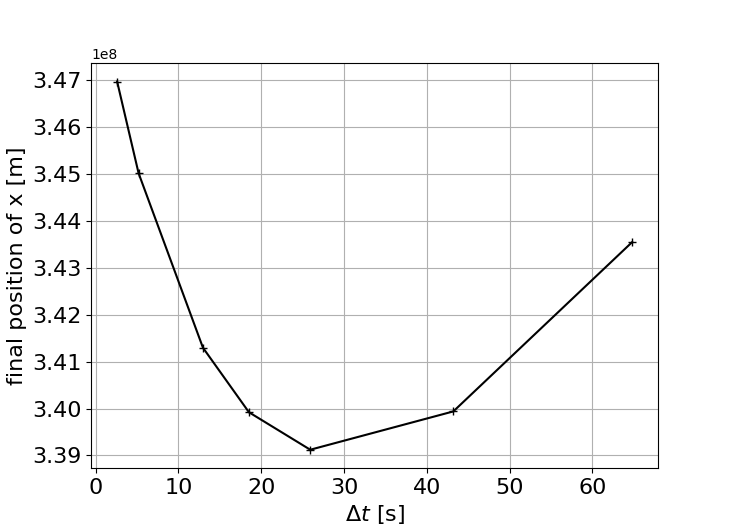
\includegraphics[scale=0.42]{Graphes/convergence_x_alpha_1.png}
    \captionsetup{justification = centering, font=large}
    \caption{}
\end{subfigure}
\hspace{0.05\textwidth}
\begin{subfigure}{0.45\textwidth}  % Réduire également ici
    \centering  % Centrer cette sous-figure
    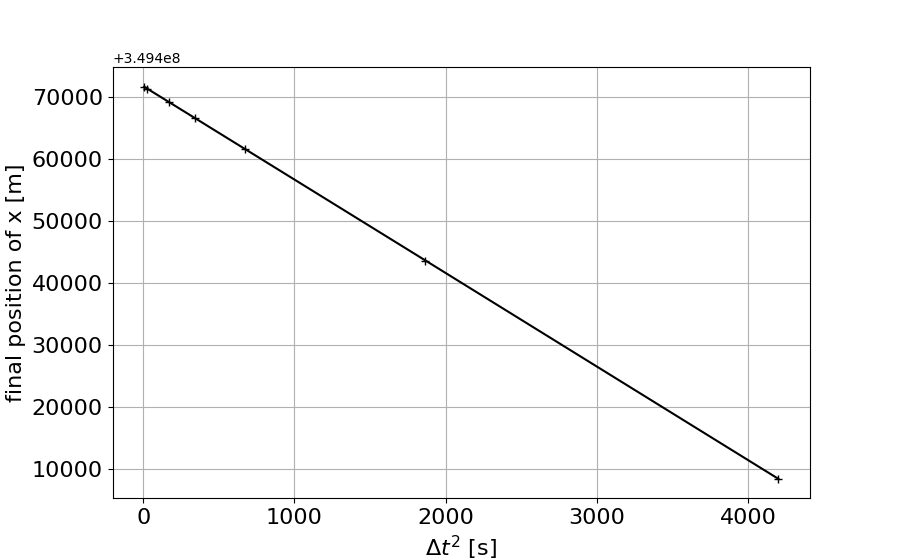
\includegraphics[scale=0.37]{Graphes/convergence_x_alpha_05.png}
    \captionsetup{justification = centering, font=large}
    \caption{}
\end{subfigure}
\captionsetup{justification=centering}
\caption{Convergence des positions finales de $x$ pour les différents schémas d'Euler : \\ (a) schéma implicite ($\alpha$ = 0), (b) schéma implicite zoomé ($\alpha$ = 0), \\ (c) schéma explicite ($\alpha$ = 1), (d) schéma semi-implicite ($\alpha$ = 0.5)}
\label{fig5}
\end{figure}

Pour les schémas explicite et implicite, les représentations des positions finales de $x'$ et $y'$ en fonction de $\Delta t$ montrent un comportement linéaire pour $\Delta t$ petit (donc $N_{steps}$ grand). Cela confirme que la convergence de ces deux schémas est d’ordre 1. Mais donc, plus $\Delta t$ est grand, moins le comportement linéaire est justifié. Pour le schéma implicite, on observe une déviation importante lors du passage trop proche de la Lune, provoquant une divergence des résultats et invalidant la convergence, alors que pour le schéma explicite, c'est sûrement l'apparition des termes quadratiques et à puissances plus élevées qui provoquent des perturbations. On remarque pour le schéma semi-implicite, la représentation des positions finales de $x'$ et $y'$ en fonction de $(\Delta t)^2$ montre une relation linéaire, indiquant une convergence d’ordre 2, ce qui montre que ce schéma est plus puissant que les schémas implicites et explicites.

\begin{figure}[H]
\begin{subfigure}{0.45\textwidth}  % Réduire la taille pour s'assurer qu'elles tiennent côte à côte
    \centering  % Centrer cette sous-figure
    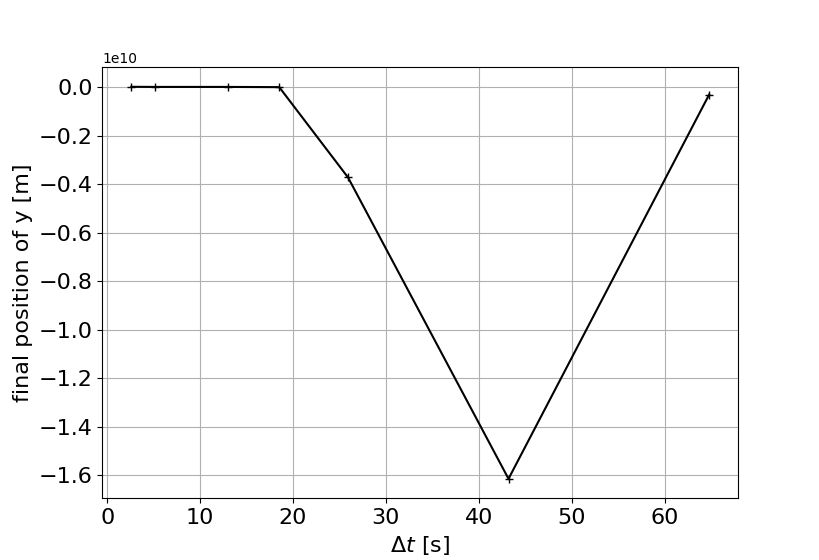
\includegraphics[scale=0.4]{Graphes/convergence_y_alpha_0.png}
    \captionsetup{justification = centering, font=large}
    \caption{}
\end{subfigure}
\hspace{0.05\textwidth}
\begin{subfigure}{0.45\textwidth}  % Réduire également ici
    \centering  % Centrer cette sous-figure
    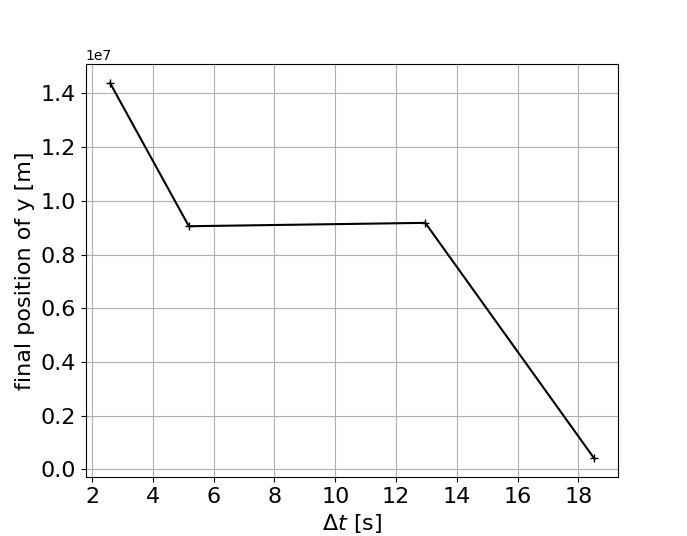
\includegraphics[scale=0.42]{Graphes/convergence_y_alpha_0_zoom.png}
    \captionsetup{justification = centering, font=large}
    \caption{}
\end{subfigure}
\begin{subfigure}{0.45\textwidth}  % Réduire la taille pour s'assurer qu'elles tiennent côte à côte
    \centering  % Centrer cette sous-figure
    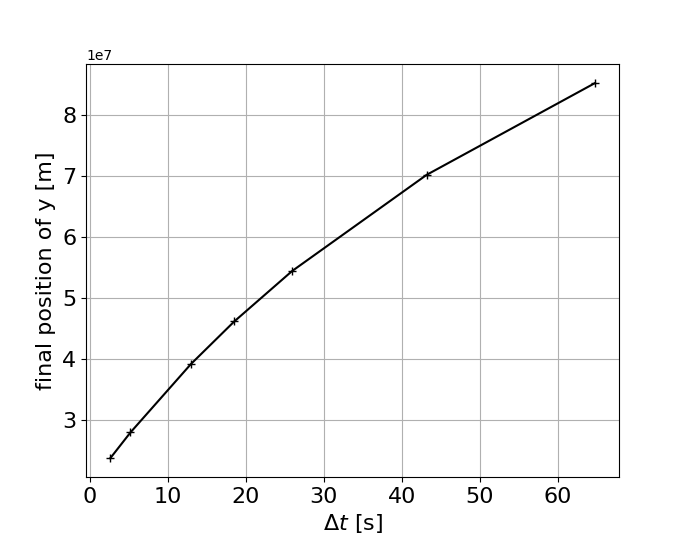
\includegraphics[scale=0.42]{Graphes/convergence_y_alpha_1.png}
    \captionsetup{justification = centering, font=large}
    \caption{}
\end{subfigure}
\hspace{0.05\textwidth}
\begin{subfigure}{0.45\textwidth}  % Réduire également ici
    \centering  % Centrer cette sous-figure
    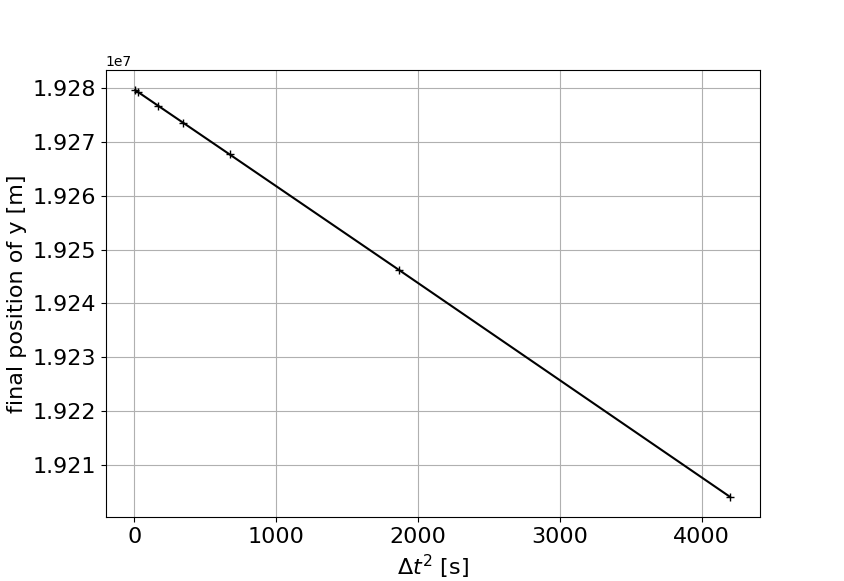
\includegraphics[scale=0.37]{Graphes/convergence_y_alpha_05.png}
    \captionsetup{justification = centering, font=large}
    \caption{}
\end{subfigure}
\captionsetup{justification=centering}
\caption{Convergence des positions finales $y$ pour les différents schémas d'Euler : \\ (a) schéma implicite ($\alpha$ = 0), (b) schéma implicite zoomé ($\alpha$ = 0), \\ (c) schéma explicite ($\alpha$ = 1), (d) schéma semi-implicite ($\alpha$ = 0.5)}
\label{fig6}
\end{figure}

Pour étudier la convergence de l'énergie mécanique, on utilise la Fig.(\ref{fig7}) montrant l'erreur de l'énergie mécanique en fonction de $N_{steps}$ dans un diagramme log-log pour différentes valeurs $N_{steps}=[2,4,6,8,10,14,20,30,50,70,100,200] \times 10^3$. Alors, la pente nous donne le degré de convergence.



\begin{figure}[H]
    \centering
    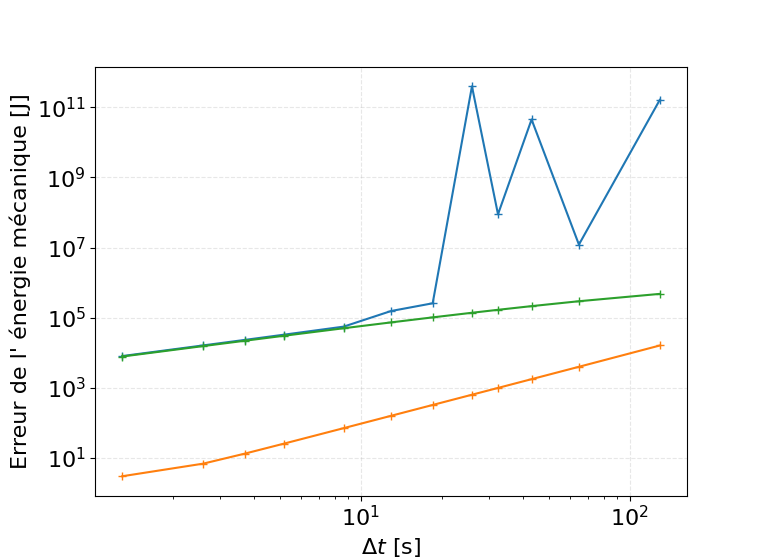
\includegraphics[width=0.6\textwidth]{Graphes/convergence_energie.png}
    \captionsetup{justification=centering}
    \caption{Erreur sur l'énergie mécanique du satellite pour les différents $N_{steps}$, avec le graphe du schéma implicite en bleu ($\alpha$ = 0), semi-implicite en orange ($\alpha$ = 0.5) et explicite en vert  ($\alpha$ = 1)}
    \label{fig7}
\end{figure}

\section{Crash-test}

On veut maintenant voir si le satellite s'écrase sur la Lune, et pour ce faire on va étudier la distance entre la Lune et le satellite au cours du temps afin de savoir si oui ou non cette distance devient inférieure au rayon de la Lune, $R_L=1737100$\,m.

En choisissant $N_{steps}=10^5$ et en prenant le schéma le plus réaliste, c'est-à-dire le schéma semi-implicite, on dresse la Fig.(\ref{fig8}) qui donne la distance étudiée en fonction du temps et on trace une ligne horizontale à $y(t)=R_L$.

\begin{figure}[H]
\begin{subfigure}{0.45\textwidth}  % Réduire la taille pour s'assurer qu'elles tiennent côte à côte
    \centering  % Centrer cette sous-figure
    \includegraphics[scale=0.5]{Crash_test.png}
\end{subfigure}
\hspace{0.05\textwidth}
\begin{subfigure}{0.45\textwidth}  % Réduire également ici
    \centering  % Centrer cette sous-figure
    \includegraphics[scale=0.5]{Crash_Test_zoom.png}
\end{subfigure}
\captionsetup{justification=centering}
\caption{Distance entre le centre de la Lune et le satellite en fonction du temps. L'image de droite présente un zoom pour mieux visualiser le moment de la collision}
\label{fig8}
\end{figure}


On voit donc que le satellite se crashe au temps $t=139650$\,s environ, ce qui fait 1 jour, 14 heures, 2 minutes et 30 secondes. On peut aussi trouver la position de crash du satellite avec la Fig.(\ref{fig9}) qui, similairement à la Fig.(\ref{fig1}), donne la trajectoire du satellite et ajoute le point de crash avec la croix orange, situé en $x=3,813 \times 10^8$\,m et $y=-1,400 \times 10^6$\,m. La ligne verticale montre les deux faces de la lune : la face visible à gauche et la face cachée à droite. On voit donc que le satellite se crash sur la face cachée de la lune.

\begin{figure}[H]
    \centering
    \includegraphics[width=0.6\textwidth]{Crash_Test_pos.png}
    \captionsetup{justification=centering}
    \caption{Trajcetoire du satellite pour $N_{steps}=100000$, avec le schéma semi-implicite, et point de contact entre la fusée et la Lune}
    \label{fig9}
\end{figure}
\vspace{-1cm}
\section{Facultatif}

Pour cette partie nous avons décidé de lancer le satellite avec une certaine vitesse $v_y$ afin que le satellite rase la Lune sans s'y écraser. Pour ce faire, nous avons repris la Fig.(\ref{fig8}), avons choisi $N_{steps}=400000$ pour être précis et avons expérimenté avec différentes vitesses initiales, comme le montre la Fig.(\ref{fig10}). La valeur empirique trouvée arrondie au centième est $v_{y,0}=-5,29$\,m/s, et donne alors que le satellite rase la Lune à une distance bien inférieure à un kilomètre !

\clearpage

\begin{figure}[H]
\begin{subfigure}{0.45\textwidth}  % Réduire la taille pour s'assurer qu'elles tiennent côte à côte
    \centering  % Centrer cette sous-figure
    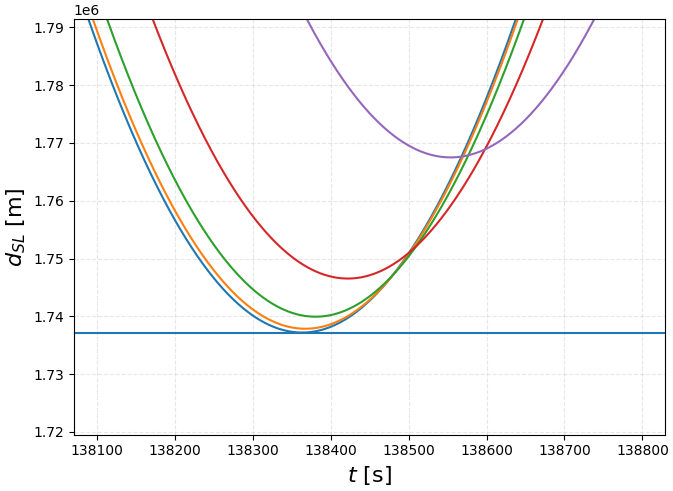
\includegraphics[scale=0.5]{Graphes/facultatif_1.png}
\end{subfigure}
\hspace{0.05\textwidth}
\begin{subfigure}{0.45\textwidth}  % Réduire également ici
    \centering  % Centrer cette sous-figure
    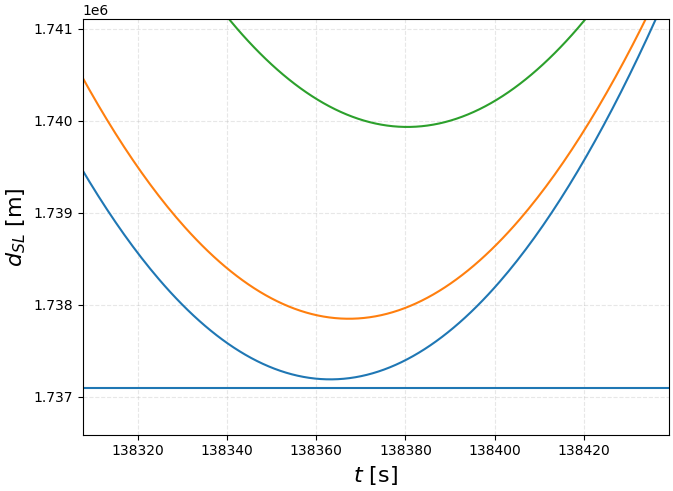
\includegraphics[scale=0.5]{Graphes/facultatif_2.png}
\end{subfigure}
\captionsetup{justification=centering}
\caption{Distance entre le centre de la Lune et le satellite en fonction du temps pour différentes valeurs $v_{y,0}$. L'image de droite présente un zoom pour mieux visualiser la distance séparant le satellite et la Lune. La courbe bleue représente $v_{y,0}=-5,29$\,m/s}
\label{fig10}
\end{figure}

\section{Conclusion}

À travers cette étude du problème à trois corps réduit, nous avons exploré et comparé les performances des schémas d’Euler explicite, implicite et semi-implicite. Chacun de ces schémas présente ses forces et ses faiblesses : tandis que les versions explicite et implicite affichent une convergence d’ordre 1, le schéma semi-implicite se distingue par une convergence d’ordre 2 et une remarquable stabilité énergétique. Finalement, notre satellite n’aura pas résisté aux lois implacables de la gravité et a terminé sa course sur la face cachée de la Lune. Ce dénouement illustre la complexité des trajectoires en mécanique céleste et la nécessité d’une approche numérique robuste pour les modéliser avec précision.


\end{document} %%%% THE END %%%%
